\section{系统测试与效果}

\subsection{测试环境}
\begin{table}[htbp]
\centering\small
\caption{测试环境}\label{tab:env}
\begin{tabular}{@{}p{4.2cm}p{9.6cm}@{}}
\toprule
硬件 & 天马F407（STM32F407ZGT6）+ ESP32-C3 核心板 + 模拟麦克风 + 3.5 寸 HX8357D\\
工具链 & F407：Keil ARMCC5 / EIDE、FreeRTOS 10.6.2；C3：ESP-IDF v5.4.4\\
烧录/调试 & OpenOCD 0.12.0 + CMSIS-DAP（SWD 500\,kHz）；esptool.py；串口助手 115\,200\\
主机侧仿真 & 2026-09-23，PC 上编译 F407 的 mic/voice/usart\_c3/proto，HAL 与对端 ACK 用桩代替，38 组通过\\
\bottomrule
\end{tabular}
\end{table}

主机仿真的原始输出在 \texttt{f407/build/voice\_host/result.log}。
测试程序直接编译上述四个 C 源文件，不跑 ESP32 固件。
399\,ms 的录音被丢弃，400\,ms 进入上传；
按住到 10\,s 得到 160000 个采样、320000 字节，上传进度走到 320000/320000，
ACK 之后桩返回文本 \texttt{raw reply: open light}，该次上传计时 3175\,ms。
同一份日志还记下 BEGIN 帧超时重试 3 次后失败、NACK 码 0x04，以及识别等待 8000\,ms 超时。
最后一行为 \texttt{PASS: 38 capture/protocol/state-machine cases}。
日志里的 \texttt{[c3]} 行只是桩打印的在线标志和 crc/ore/drop 计数。
这次等待时限按当时源码是 8\,s；当前固件的识别等待已改为 30\,s，两处不要混成同一次配置。

测试遵循``每步独立通过标准''的联调顺序：屏幕与界面 $\to$ 传感器 $\to$ C3 独立联网
$\to$ 双板帧链路 $\to$ 语音全链路 $\to$ 断网降级。以下逐模块给出方法与结果。

\subsection{分模块测试}
\subsubsection{界面与走时}
下面几张是按当前 LVGL 页面生成的界面示意图，不是实机拍摄。
图中的时刻、步数和天气是排版用的样子。主页是六行列表，第一行处于选中态。
\begin{figure}[htbp]
\centering
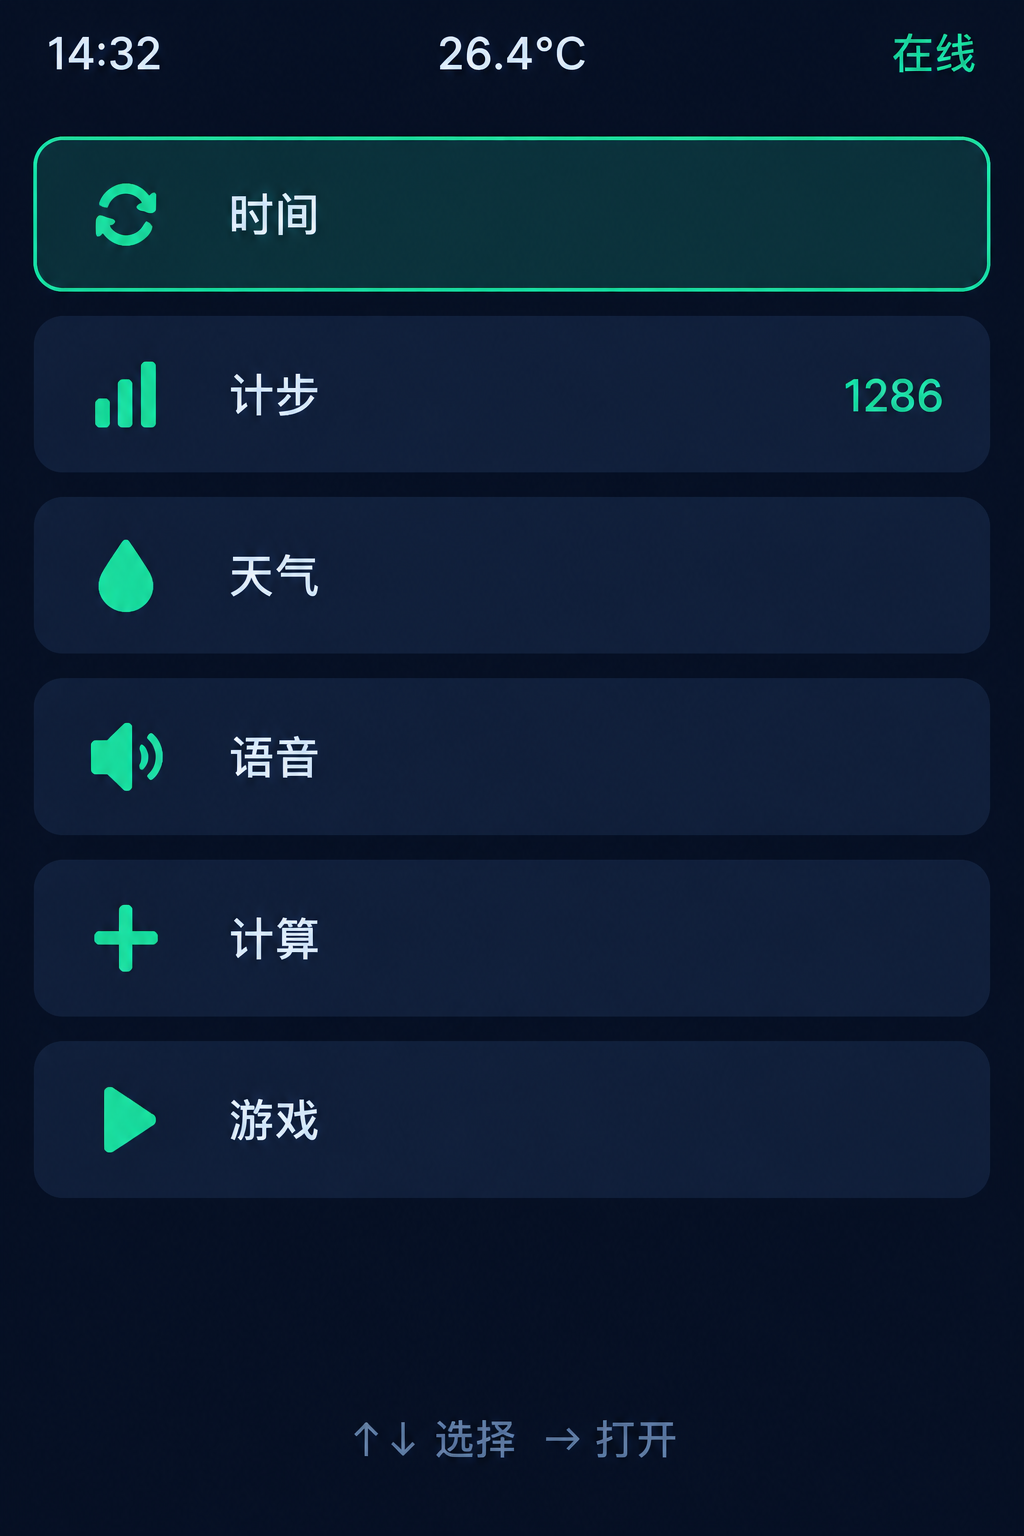
\includegraphics[width=0.36\linewidth]{picture/01.png}
\caption{主页示意图}\label{shot:home}
\end{figure}
\begin{figure}[htbp]
\centering
\includegraphics[width=0.36\linewidth]{"picture/01 (1).png"}\hfill
\includegraphics[width=0.36\linewidth]{"picture/01 (2).png"}
\caption{时间页与计步页示意图}\label{shot:time}
\end{figure}

\subsubsection{传感器与计步}
计步页已见图~\ref{shot:time}。天气页同样是示意图，摘要文字不是实测气象。
\begin{figure}[htbp]
\centering
\includegraphics[width=0.36\linewidth]{"picture/01 (3).png"}
\caption{天气页示意图}\label{shot:weather}
\end{figure}

\subsubsection{C3 串口日志}
2026-09-24 的 C3 控制台原文保存在 \texttt{dialogue\_uart.log}。\newline
固件版本是 \texttt{c3-dialogue-10s-1}。\newline
编译时间是 2026-09-24 01:16:50，ELF 校验前缀是 \texttt{adcc25215}。
启动横幅给出 UART1 为 460800\,8N1，发送脚 GPIO4，接收脚 GPIO5，
音频暂存分区 393\,216 字节、上限 320\,000 字节，启动时空闲堆 257\,264 字节。
Wi-Fi 先以 reason 4、reason 205 断开，约 5\,s 后重连，取得地址 10.95.230.254。
这条日志没有天气查询的 HTTP 记录。

\subsubsection{语音全链路}
同一份串口日志里有两段短录音，都短于 10\,s 上限。第一轮收齐后完成上云；
上传过程中又来的 BEGIN 被拒绝。第二轮只记到证书校验，文件在此结束。
\begin{table}[htbp]
\centering\small
\caption{2026-09-24 C3 串口日志中的两段语音}\label{tab:voicetest}
\begin{tabular}{@{}lcc@{}}
\toprule
项目 & 第一轮 & 第二轮\\
\midrule
PCM & 44\,502\,B & 81\,400\,B\\
串口收齐 & 1\,551\,ms & 2\,817\,ms\\
WAV & 44\,546\,B & 81\,444\,B\\
请求体 & 59\,833\,B & 109\,029\,B\\
云端 & HTTP 200 & 止于证书校验\\
HTTPS 发送 & 11\,849\,ms & 本日志没有\\
空闲堆 & 187\,740\,B & 188\,668\,B\\
\bottomrule
\end{tabular}
\end{table}
第一轮模型回复为「你好呀～请问有什么我可以帮到你的吗？」。
第二轮的 188\,668 字节是开始上传前的空闲堆。
图~\ref{shot:voice} 按该回复画了语音页，属于界面示意图。
\begin{figure}[htbp]
\centering
\includegraphics[width=0.36\linewidth]{"picture/01 (4).png"}
\caption{语音页示意图}\label{shot:voice}
\end{figure}

\subsubsection{断网降级}
关闭路由器后，状态栏右侧应由绿色「在线」改为橙色「离线」。
再按住上键时，语音页返回未联网错误（0x03）；时钟、计步和表温仍继续工作。
本报告没有单独的离线示意图。

\subsection{资源占用}
\begin{table}[htbp]
\centering\small
\caption{资源占用实测}\label{tab:resource}
\begin{tabular}{@{}llp{8.2cm}@{}}
\toprule
平台 & 资源 & 占用\\
\midrule
F407 & 代码 & 约 245\,KB\\
F407 & Flash 执行区 & 约 836\,KB / 1\,MB，其中汉字字库约 475\,KB\\
F407 & 片内 RAM & 约 105.5\,KB / 128\,KB\\
F407 & 外部 SRAM & 录音缓冲 320\,000\,B\\
C3 & 空闲堆 & 约 187\,KB\\
C3 & audio 分区 & 384\,KB，存放最长 10\,s 的 PCM\\
\bottomrule
\end{tabular}
\end{table}

\subsection{调试问题与解决过程}
调试过程记录三个有代表性的问题，全部来自真实联调，解决方式均为根因修复。

\textbf{问题一：外部 SRAM 写入偶发读回错误。}
连续录音时外扩 SRAM 出现两次 PCM 写后读校验拦截（错误码 0x20）。
排查发现 SRAM 的 FSMC 引脚配置遗漏（NE3/PG10、NBL0/NBL1/PE0/1 未初始化），
补齐引脚后仍有偶发错误，进一步把 Bank3 地址建立时间加到 3、数据建立 12 个 HCLK，
数据阶段余量约 77\,ns 后彻底消除。这一问题被自研的``写后读校验''机制当场拦截，
未产生上云的坏数据。

\textbf{问题二：复位后进入系统 Bootloader。}
一次普通复位后采样向量表，发现 MSP/PC 指向系统 ROM（0x1FFF3DA1）而非 Flash 应用，
应用未启动。逐项核对 BOOT 跳线：BOOT0 与 GND 短接确认、BOOT1 的 GND 跳线帽
脱落已补回；但补回后该次复位仍进 ROM。判断 BOOT1 与本现象无关，
真正原因是该次采样时刻 BOOT0 实际电平未被证明——USB 的 CH340 自动下载电路
亦连接 BOOT0。以调试器恢复 Flash 向量映射与 VTOR 后应用正常运行。

\textbf{问题三：板上镜像与磁盘源码不一致。}
实板日志打印的字符串既不在磁盘 C3 源码中、也不在当前构建产物中，
且 C3 收到音频帧后只回 ACK 而无云端动作——板上运行的是一份旧版固件。
据此建立了 ELF SHA-256 启动横幅自检机制，并明确``ACK 只代表帧被应答，
不代表云端请求成功''的日志语义。

\subsection{结果分析}
对照指导书要求：数据采集、本地处理与控制、GUI 显示、云端交互四项功能全部打通；
可靠性方面帧协议在两轮实测中零 CRC/零溢出/零丢帧；
断网降级行为符合设计预期。

局限与未完成项：
\begin{enumerate}[label=（\arabic*）]
\item 语音识别率未做定量验收，没有多人次、多词条的统计。
\item 麦克风存在直流偏置。录音 ADC 均值约 156，低于换算假定的中点 2048，
去均值后交流幅度偏小，云端能否听清取决于说话音量。软件里还没有去直流和增益。
\item 满 10\,s 的录音这条串口日志里没有。2026-09-24 上板的是
\texttt{c3-dialogue-10s-1}，两段都是短录音。F407 侧 10\,s 满长只做过 9 月 23 日的主机仿真。
\item 跌倒告警的 C3 上报路径（0x30 帧）已定义，尚未启用。当前只有本地蜂鸣和告警页。
\end{enumerate}
